
%
% template for Bachelor thesis
% LIACS
% January 7, 2019
%

\documentclass[12pt]{article}

% include some packages
\usepackage[left=2cm,right=2cm,top=2cm,bottom=3cm]{geometry}
\usepackage{graphicx}
\usepackage{tikz}
\usetikzlibrary{shapes,backgrounds,calc,arrows}
\usepackage{microtype}
\usepackage{amsmath}
\usepackage[utf8]{inputenc}
\usepackage{amsfonts}
\usepackage{amssymb}
\usepackage{amsthm}
\usepackage{bbm}
\usepackage{geometry}
\usepackage{csquotes}
\usepackage[hidelinks]{hyperref}
\usepackage{mathtools}
\usepackage{parskip}

\usepackage{mathtools}
\newcommand{\defeq}{\vcentcolon=}
\newcommand{\eqdef}{=\vcentcolon}

\DeclareMathOperator{\Ima}{Im}
\DeclareMathOperator{\sech}{sech}
\renewcommand{\P}{\mathcal{P}}
\newcommand{\R}{\mathbb{R}}
\newcommand{\C}{\mathbb{C}}
\newcommand{\N}{\mathbb{N}}
\newcommand{\E}[1]{\mathbb{E}\{#1\}}
\newcommand{\Q}{\mathbb Q}
\newcommand{\Z}{\mathbb{Z}}
\newcommand{\1}{\mathbbm{1}}
\newcommand{\ua}{\nearrow}
\newcommand{\da}{\searrow}
\newcommand{\eps}{\varepsilon}
\newcommand{\dx}{\mathrm{d}x}
\newcommand{\B}{\mathcal{B}}
\newcommand{\F}{\mathcal{F}}
\newcommand{\T}{\mathbb{T}}
\newcommand{\V}{\mathcal{V}}
\newcommand{\U}{\mathcal{U}}
\newcommand{\id}{\text{id}}
\newcommand{\I}{\mathcal{I}}
\newcommand{\A}{\mathcal{A}}
\newcommand{\J}{\mathcal{J}}
\newcommand{\G}{\mathcal{G}}
\renewcommand{\L}{\mathcal{L}}
\newcommand{\specepsilon}{\mathcal{E}}
\newcommand{\M}{\mathcal{M}}
\newcommand{\II}{\textbf{II}}
\newcommand{\bigo}{\mathcal{O}}
\usepackage[setpagesize=false,colorlinks=true,linkcolor=blue,urlcolor=red,pdftitle={An Interesting Title for a Thesis},pdfauthor={Your Name}]{hyperref}
\setlength\parindent{0pt}

\begin{document}
\thispagestyle{empty}


\includegraphics{logoleiden}

\vspace{-2.5cm}\hfill \begin{huge}\textbf{Opleiding Informatica}\end{huge}

\vspace{5cm}
\begin{Large}
\hfill Simplicial Coalgebras

\vspace*{3mm}

\hfill for Concurrent Regular Languages

\vspace*{14mm}

\hfill Hessel Sieburgh
\end{Large}

\vspace*{6.0cm}

\begin{large}

Supervisors:\\
Henning Basold \& 
Marton Hablicsek


\vspace*{2.8cm}
BACHELOR THESIS

\vspace*{5mm}
Leiden Institute of Advanced Computer Science (LIACS)\\
\href{www.liacs.leidenuniv.nl}{\underline{\texttt{www.liacs.leidenuniv.nl}}}\hfill 01/07/2025
\end{large}

\newpage



% abstract and references should fit on one page
\begin{abstract}
\noindent
This is where you write an abstract that concisely summarizes your thesis.
Keep it short. No references here --- exceptions do occur.
\end{abstract}

\bigskip

\thispagestyle{empty}
\tableofcontents
\thispagestyle{empty}
%Some (very few) people like a list of tables:
%\listoftables
%And some (even fewer) like a list of figures:
%\listoffigures

\clearpage
\setcounter{page}{1}

\section{Introduction} \label{introduction}

In this section we give an introduction to the problem addressed in this thesis.


\subsection{The situation}

Sections may include subsections.

To make sure that this document renders correctly, execute these commands:
\begin{quote}
\begin{verbatim}
pdflatex thesis
bibtex thesis
pdflatex thesis
pdflatex thesis
\end{verbatim}
\end{quote}
Here, the \verb|pdflatex| command may need to be executed three times in order to generate the table of contents and so on. 
Note that a good thesis has figures and tables; examples can be found in Figure~\ref{afigure} and Table~\ref{atable}. And every thesis has references, like~\cite{whatagreatpaper}.

\begin{figure}[!htbp]
\begin{center}
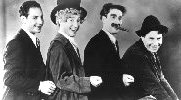
\includegraphics[height=2cm]{marxbrothers2}
\end{center}
\caption{Every thesis should have figures. Source: \href{www.marxbrothers.org}{\underline{\texttt{www.marxbrothers.org}}}.}\label{afigure}
\end{figure}

\begin{table}[!htbp]
\begin{center}
\begin{tabular}{l|l}
Column A & Column B\\
\hline
Point 1 & Good\\
Point 2 & Bad
\end{tabular}
\end{center}
\caption{Every thesis should have tables.}\label{atable}
\end{table}

Final reminder: this template is just an example, if you want you can make adjustments; also discuss with your supervisor which layout he or she likes. But the front page should be as it is now.

TODO: quite a lot!

\subsection{Thesis overview}
It is recommended to end the introduction with an overview of the thesis. This chapter contains the introduction; Section~\ref{definitions} includes the definitions; Section~\ref{relatedwork} discusses related work; Section~\ref{experiments} describes the experiments and their outcome; Section~\ref{conclusions} concludes. By the way, different section titles are certainly possible.

Also, produce a nice sentence with ``bachelor thesis'', LIACS and the names of the supervisors.

\section{Notes}\label{notes}
\paragraph{Connected components}
Let $S$ be a simplicial set with an iPomset label set $L$ and a labeling map $\ell: S \rightarrow L$. Say that $x,y\in S$ are \textit{iPomset neighbors} iff there is a face map from one to the other, and $\ell(x)$,$\ell(y)$ are equal when disregarding event order.

This gives us path connected components of $S$ where $x\sim y$ (are connected) iff there is a path of neighbors connecting $x$ and $y$.

In this way (when denoting simplicial set elements by their labels)\[
\begin{pmatrix} a \\ b \end{pmatrix}
\sim 
\{a,b\}
\sim
\begin{pmatrix} b \\ a \end{pmatrix}
\]
 in the figure below.
\begin{figure}[h]
    \centering
    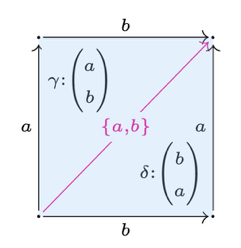
\includegraphics[width=0.3\linewidth]{image.png}
    \caption{equivalence of iPomsets}
    \label{fig:ipomset-equivalence}
\end{figure}

We then take the quotient over this relation to get something workable for a transition coalgebra:
\[
    H \defeq S/\sim
\]

We can partition this into $H = H_1 \sqcup H_2 \sqcup H_3, \dots$ Where $[x]_{\sim} \in H_k$ iff its shared iPomset event set contains $k$ events.
This also entails that if $[x]\in H_k$ then the maximum dimension of an element of $[x]$ is $k$.

We first intuitively look at what happens when we transition. From each state (class) in $H$ we have maps 
What we can then do to transition is as follows:
Let the current state of the system be $[x]_{\sim}\in H_k$, the equivalence class of some $x\in S$ under $\sim$, from here on written as $[x]$.
\newpage

Define the transition maps $\downarrow_a^k: H_k\to H_{k-1}$ and $\uparrow_a^k: H_k \to H_{k+1}$ as follows:

\begin{itemize}
    \item The \textit{downward transition} map $\downarrow_a^k$ represents the transition when action $a$ ends:
    \[
    \downarrow_a^k: [x] \mapsto [y]
    \]
    iff there are $x'\in [x]$, $y'\in [y]$ for which there exists a face map $d_i: x' \to y'$ in $S$ such that
    \[
    P_{[y]} = P_{[x]} \setminus \{a\}.
    \]
    where $P_{[x]}$ denotes the event set of $\ell(x)$
    
    \item The \textit{upward transition} map $\uparrow_a^k$ represents the transition when action $a$ begins:
    \[
    \uparrow_a^k: [x] \mapsto [y]
    \]
    iff $\downarrow_a^{k+1}([y]) = [x]$, which therefore adds $a$ to the currently running events: 
    \[
    P_{[y]} = P_{[x]} \cup \{a\}.
    \]
\end{itemize}

Now the directionality of a HDA can be easily constructed. It is simply a choice of allowed which will then define our coalgebra.
\newpage
\section{Related Work}\label{relatedwork}

\section{Experiments}\label{experiments}

\section{Conclusions and Further Research}\label{conclusions}

\bibliographystyle{alpha}
\bibliography{bibliography}
\addcontentsline{toc}{section}{References}


%\appendix
%appendices here --- if any

\end{document}
